\documentclass[aspectratio=169,10pt]{beamer}
\usetheme{Madrid}
\usecolortheme{seahorse}
\usefonttheme{professionalfonts}
\usepackage{fontspec}
\setmainfont{TeX Gyre Pagella}
\setsansfont{TeX Gyre Heros}
\setmonofont{TeX Gyre Cursor}
\usepackage{amsmath}
\usepackage{tikz}
\title{Overlay behaviour}
\subtitle{Pauses, covers and themes}
\author{Ratex Fixtures}
\institute{Typesetting Lab}
\date{Fixed date}

\begin{document}
\begin{frame}
  \titlepage
\end{frame}
\begin{frame}{Outline}
  \tableofcontents
\end{frame}

\section{Incremental content}
\begin{frame}{Itemized reveal}
  \begin{itemize}[<+->]
    \item First stage arrives alone
    \item Second stage follows
    \item Third stage completes the list
  \end{itemize}
  \pause
  \alert{Alerted summary appears last.}
\end{frame}

\begin{frame}{Covers and only}
  \uncover<2->{Uncovered from slide two.}\par
  \only<1>{Only on slide one.}\only<2>{Only on slide two.}\only<3>{Only on slide three.}\par
  \visible<3>{Visible on slide three.}\par
  \textbf<2>{Bold on the second slide.}
\end{frame}

\section{Math and graphics}
\begin{frame}{Blocks and columns}
  \begin{columns}[T]
    \begin{column}{.48\textwidth}
      \begin{block}{Quadratic}
        \[x=\frac{-b\pm\sqrt{b^{2}-4ac}}{2a}\]
      \end{block}
      \begin{exampleblock}<2->{Example}
        With $a=1,b=-3,c=2$ we get $x\in\{1,2\}$.
      \end{exampleblock}
    \end{column}
    \begin{column}{.48\textwidth}
      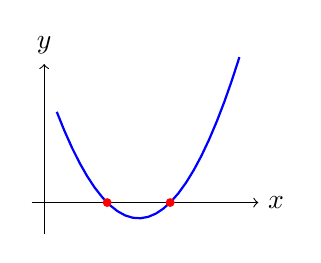
\begin{tikzpicture}[scale=.8]
        \draw[->] (-.2,0)--(3.4,0) node[right]{$x$};
        \draw[->] (0,-.5)--(0,2.2) node[above]{$y$};
        \draw[blue,thick,domain=0.2:3.1] plot (\x,{(\x-1)*(\x-2)});
        \visible<2->{\fill[red] (1,0) circle (2pt) (2,0) circle (2pt);}
      \end{tikzpicture}
    \end{column}
  \end{columns}
\end{frame}
\begin{frame}[fragile]{Verbatim in a fragile frame}
  \begin{verbatim}
\only<1>{a}\only<2>{b}
  \end{verbatim}
  \texttt{\textbackslash alert} marks \alert{emphasis}.
\end{frame}
\end{document}
